\newpage
\section{Spanner: A Globally-Distributed Database}
In 2012, Corbett et al. introduced Spanner, Google's scalable, multi-version, globally-distributed, and synchronously-replicated database.
The first system to support world-wide atomic transactions with its novel TrueTime API (\href{https://static.googleusercontent.com/media/research.google.com/en//archive/spanner-osdi2012.pdf}{Original Paper}):

\vspace{2em}
\begin{Def}[Spanner Design Goals]

    Google's Spanner is architected to be a planet-scale, strongly-consistent system.  Its primary design goals are:
    
    \begin{itemize}
      \item \textbf{Global Scale \& Distribution:} Span millions of machines and petabytes of data across multiple datacenters, automatically sharding and rebalancing data.
      \item \textbf{External Consistency:} Provide linearizable reads and writes across shards and datacenters via TrueTime; every transaction appears to occur at a single, globally-agreed timestamp.
      \item \textbf{Serializability:} Support serializable multi-row, multi-shard transactions using two-phase locking within Paxos-replicated groups (a consensus model comparable to raft) and two-phase commit across groups.
      \item \textbf{High Availability \& Durability:} Synchronously replicate each shard with Paxos so that any replica group tolerates datacenter outages without losing committed data.
      \item \textbf{Low-Latency, \underline{Lock-Free Reads}:} Enable read-only transactions to serve at a timestamp in the past without acquiring locks, minimizing read latency under contention.
    \end{itemize}

    \noindent
    In short,\\
    \textbf{Consistency Model:} Strict serializability, with atomic transactions.
    \end{Def}
    
    \begin{Note}
    \textbf{Note:} We do not cover paxos, but every time it is said, just think of it as the consensus module in the system. I.e., one may 
    synonymously think of it as raft.
    \end{Note}
    \noindent
    The main motivation here is that when we want to do a database backup, or perform some enourmous read, placing a lock on the entire system would not be a 
    great user experience. So we utilize snapshots instead, recall Definition (\ref{def:consistency}):

    \newpage 

    \noindent
    Let's discuss how Spanner achieves these goals, with snapshots and timestamps:
    \begin{Def}[Consistent Snapshots via MVCC]

        \label{def:spanner}
        Spanner uses \textbf{Multi-Version Concurrency Control (MVCC)} and globally ordered timestamps to serve lock-free, causally-consistent read-only transactions:
        
        \begin{itemize}
          \item \textbf{Versioned Writes:} Each update transaction $T_w$ is assigned a unique, monotonically increasing commit timestamp $t_w$.  Every write to key $k$ creates a new version tagged with $t_w$ rather than overwriting.
          \item \textbf{Safe Time Rule:} Before $T_r$ reads key $k$, it must see a write $T_w$ that is $t_w > t_r$.
          \item \textbf{Causal Consistency:} Global timestamp ordering ensures that if $T_1\to T_2$, any snapshot that reflects $T_2$'s writes also reflects $T_1$'s.
          \item \textbf{Lock-Free Reads:} Read-only transactions never acquire locks and run entirely against their fixed snapshot, eliminating read-write contention.
        \end{itemize}
        \end{Def}
        
        \noindent
    \noindent
    
    \begin{Def}[Commit Timestamp Ordering]
        
        Spanner assigns each transaction \(T_i\) a commit timestamp \(t_n\) s.t., for any two \(T_1\) and \(T_2\):
        \[
        T_1 \text{ completes before } T_2 \quad\Longrightarrow\quad t_1 < t_2.
        \]
        \noindent
        We use \textbf{physical clocks} (atomic) to assign timestamps. Lamport (logical) clocks capture causal dependencies but \textbf{do not guarantee} real-time precedence.
        \end{Def}
    \begin{figure}[ht!]
        \centering
        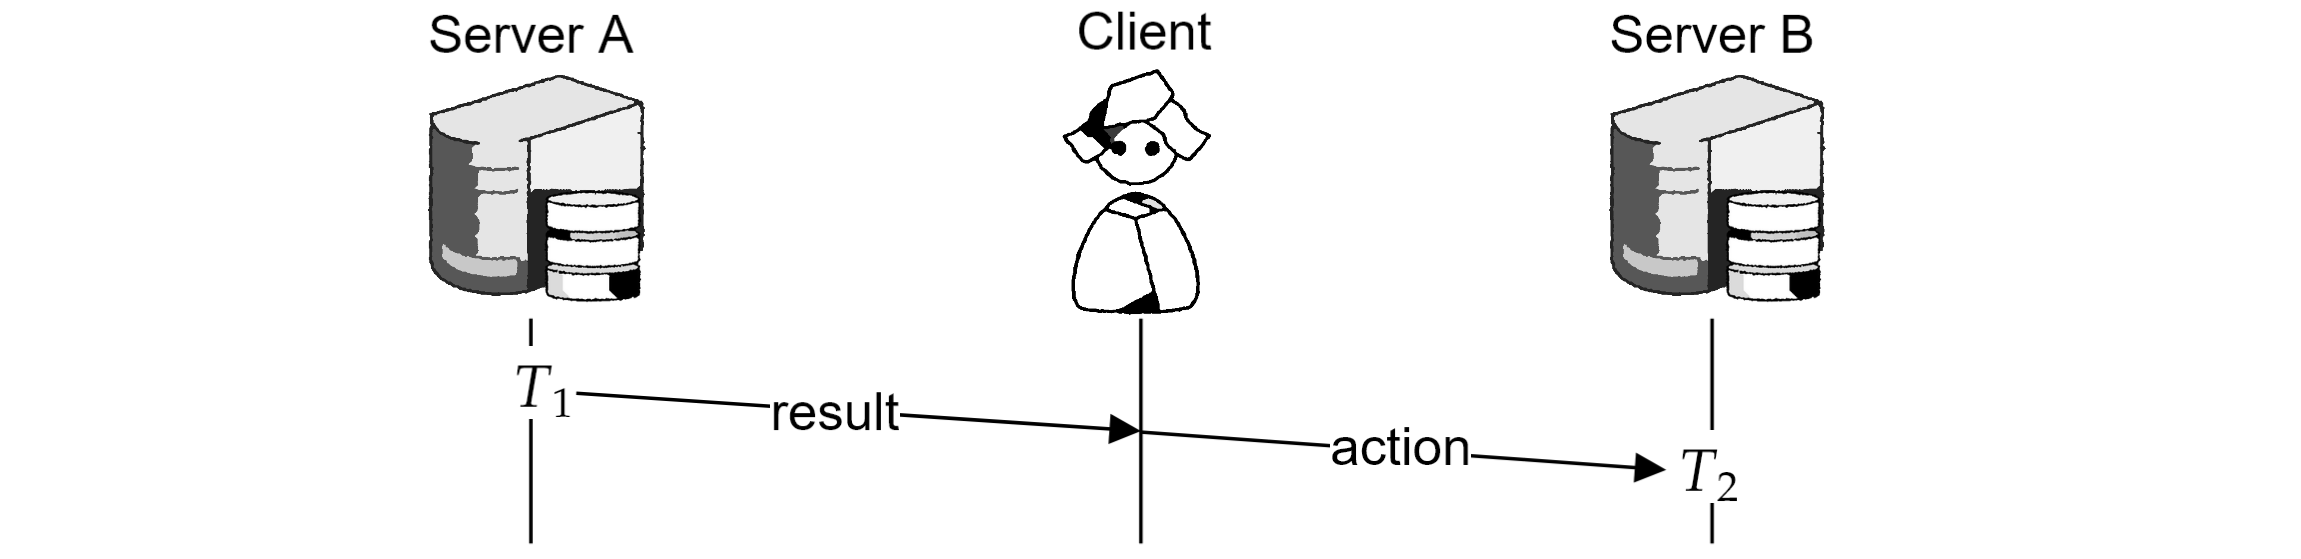
\includegraphics[width=\textwidth]{Sections/span/tt.png}
        \caption{Server $A$ may never communicate with server $B$, making logical clocks insufficient.}
    \end{figure}
        
\newpage 
\noindent
Google implements atomic clocks and GPS receivers to mitigate physical limitations of clocks:
\begin{Def}[TrueTime: Bounded Clock Uncertainty]

    Spanner's TrueTime API provides each server a timestamp interval
    \([t_{\mathit{earliest}},\,t_{\mathit{latest}}]\) such that the actual absolute time (real-time) \(t_{\mathit{abs}}\) lies within the interval:
    \(
    t_{\mathit{earliest}} \;\le\; t_{\mathit{abs}}\;\le\; t_{\mathit{latest}}
    \).
    On commit, Spanner enforces strict real-time ordering by:
    
    \begin{itemize}
      \item \textbf{Interval Return:} A call to \(\mathtt{TT.now()}\) returns \([t_{\mathit{earliest}},t_{\mathit{latest}}]\).
      \item \textbf{Uncertainty Wait:} Before finalizing a commit timestamp \(t\), the coordinator waits until its local clock \(\ge t_{\mathit{latest}}\), ensuring no future transaction can obtain a timestamp \(\le t\).
      \item \textbf{Monotonicity \& Ordering:} This wait ensures that once a transaction reports commit at \(t\), all subsequent \(\mathtt{TT.now()}\) calls on any server will yield intervals with \(t_{\mathit{earliest}}>t\), guaranteeing \(T_1\) commit precedes \(T_2\) timestamp.
      \item \textbf{Global Coverage:} By combining redundant GPS receivers and local atomic clocks in each datacenter, TrueTime keeps its uncertainty bound \(\delta = t_{\mathit{latest}} - t_{\mathit{earliest}}\) small (typically a few milliseconds), even under network partitions (Kops)
    \end{itemize}

    \noindent
    E.g., If it's 12:32:01 pm we might see: [12:31:59pm, 12:32:04pm] where $\delta$ is 5 milliseconds.
    \end{Def}

    \begin{figure}[ht!]

        \centering
        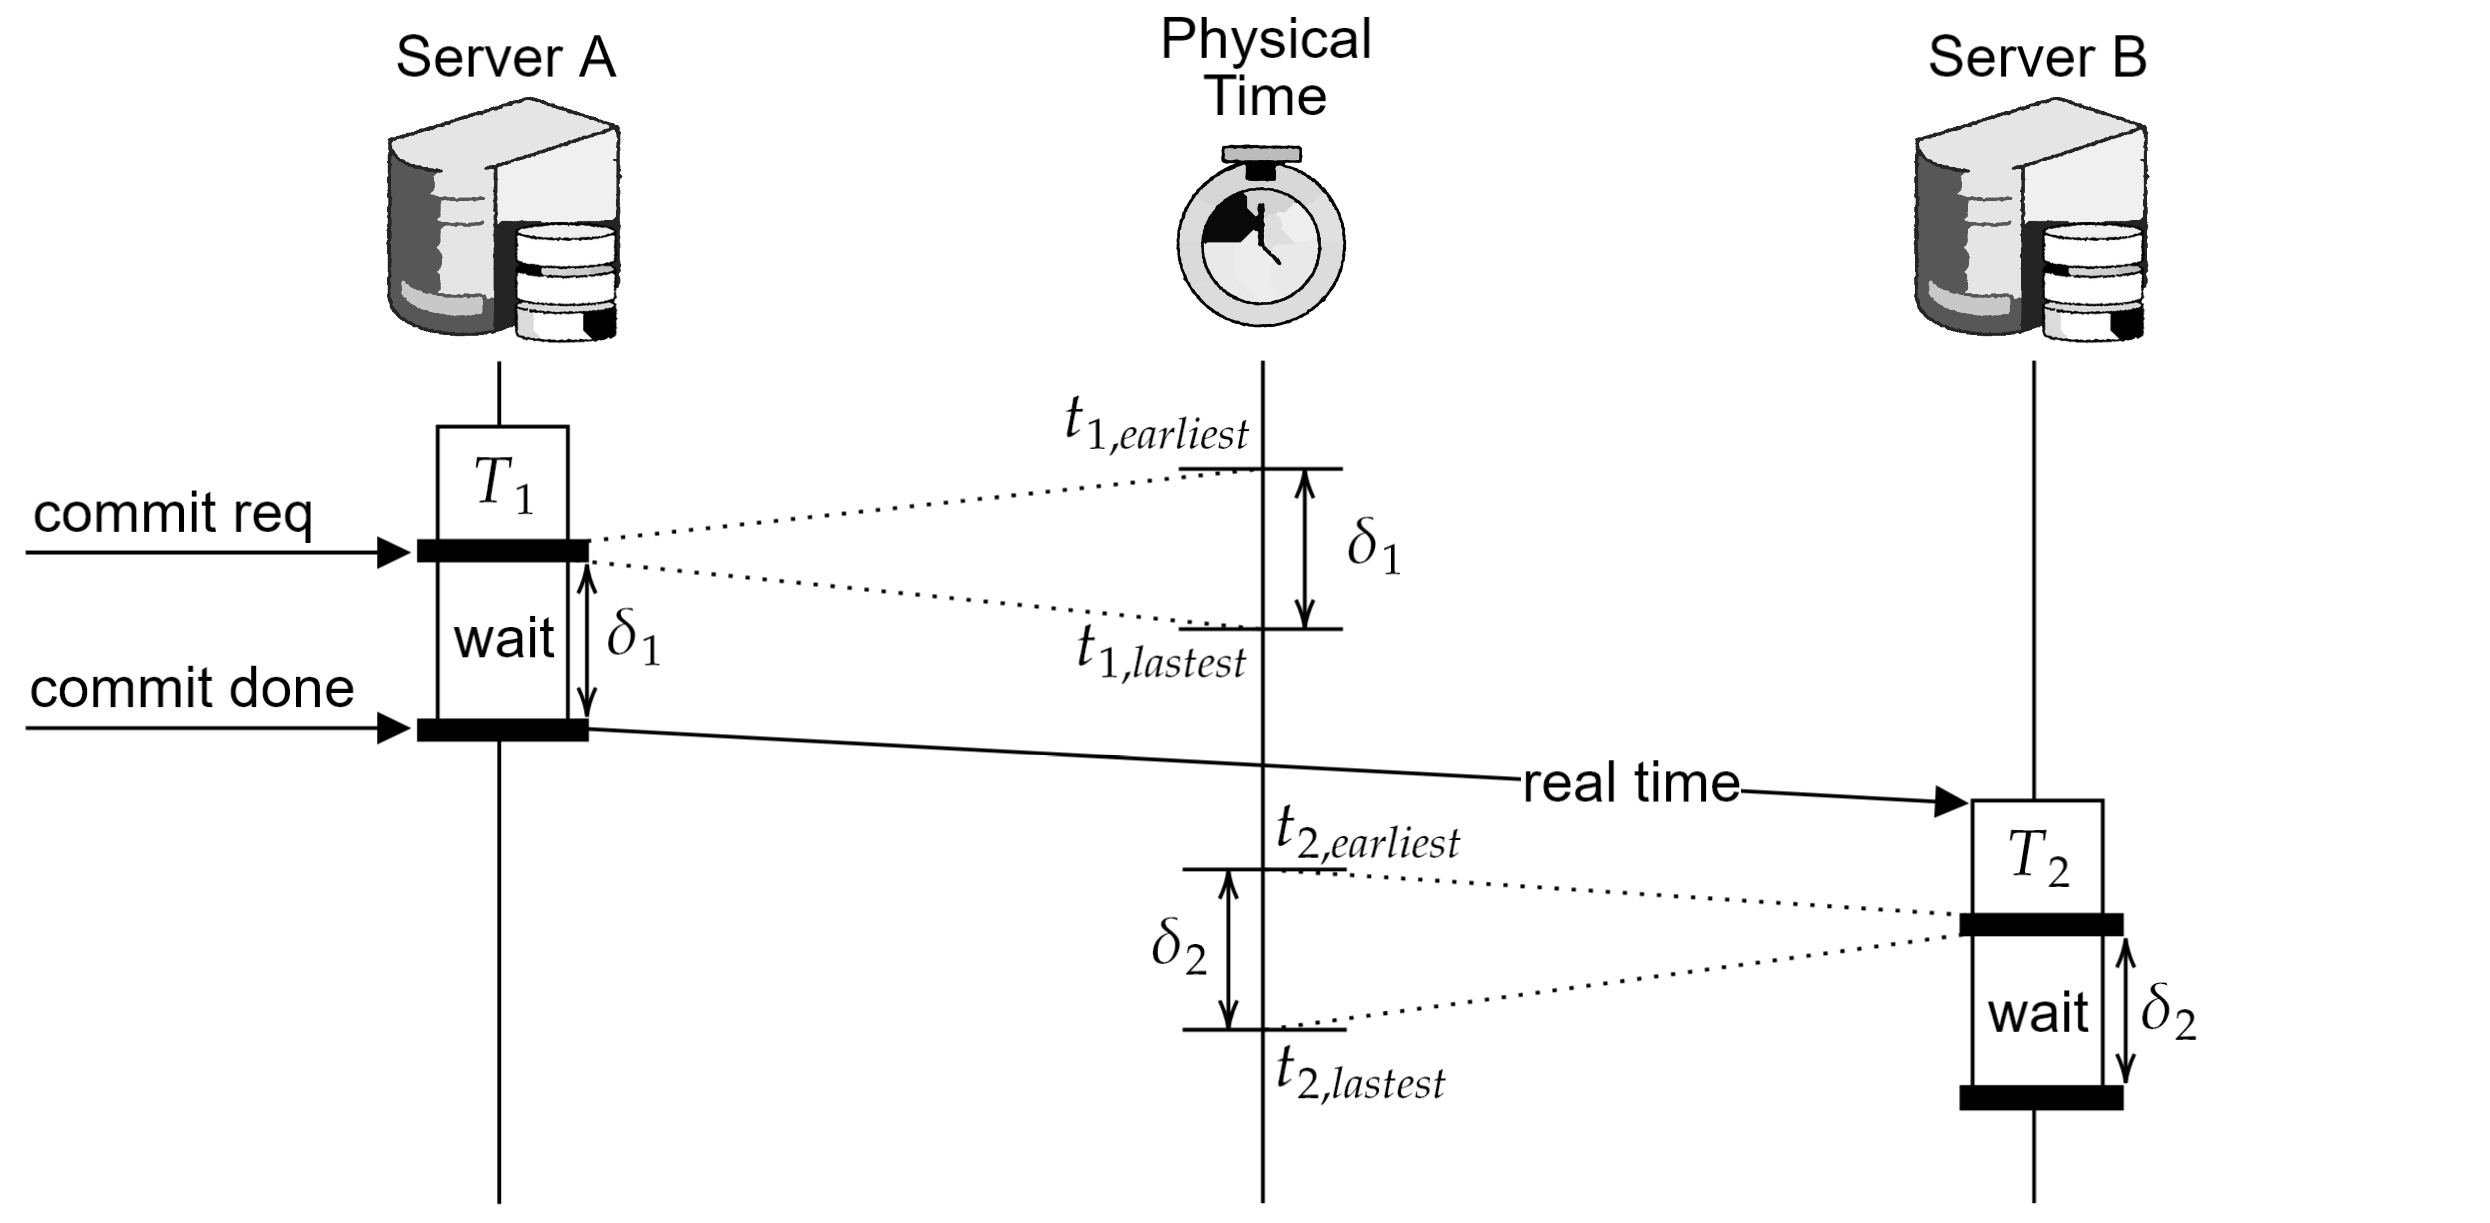
\includegraphics[width=\textwidth]{Sections/span/tt_2.png}
        \caption{Upon receiving a commit request, each coordinator (e.g.\ A) calls \texttt{TT.now()} and obtains an uncertainty interval \([t_{1,\mathrm{earliest}},\,t_{1,\mathrm{latest}}]\). It then delays for \(\delta_1 = t_{1,\mathrm{latest}} - t_{1,\mathrm{earliest}}\) before finalizing its commit timestamp.}
    \end{figure}

    \newpage 

    \noindent
    Finally we touch on the two-phase commit protocol:

    \begin{Def}[Cross-Shard Transactions \& Paxos Replication]

        Spanner provides strictly serializable, atomic transactions across independently-replicated shards by combining two-phase locking (2PL), two-phase commit (2PC), and Paxos state-machine replication:
        
        \begin{itemize}
          \item \textbf{Coordinator Selection:}  
            After a client buffers all its reads and pending writes, it picks one of the involved shards' Paxos group leaders to act as the \textbf{2PC coordinator}.  
            This is simply the leader replica for one of the keys in the transaction's shard set.  
          \item \textbf{Intra-Shard Isolation:}  
            Within each shard, that shard's Paxos leader acquires two-phase-locks on the keys being accessed, serializing concurrent read-write operations.
          \item \textbf{Atomic Cross-Shard Commit:}  
            The coordinator issues a 2PC ``\texttt{PREPARE}'' to every participant leader. Each participant logs the prepare record via Paxos, acquires its write-locks, and returns a prepare-OK.  
            Once the coordinator has all prepares, it logs the global ``\texttt{COMMIT}'' via Paxos to each shard, ensuring the transaction is made durable and atomic.
          \item \textbf{Paxos Fault Tolerance:}  
            Let $f$ be the maximum number of servers allowed to fail before system failure. Then each shard is a Paxos group of \(n=2f+1\) replicas; as long as a majority (\(f+1\)) are up, Paxos ensures progress, automatically electing new leaders and replicating log entries even if up to \(f\) replicas fail.
           
        \end{itemize}
        \end{Def}
        
\begin{figure}[ht!]
    \centering
    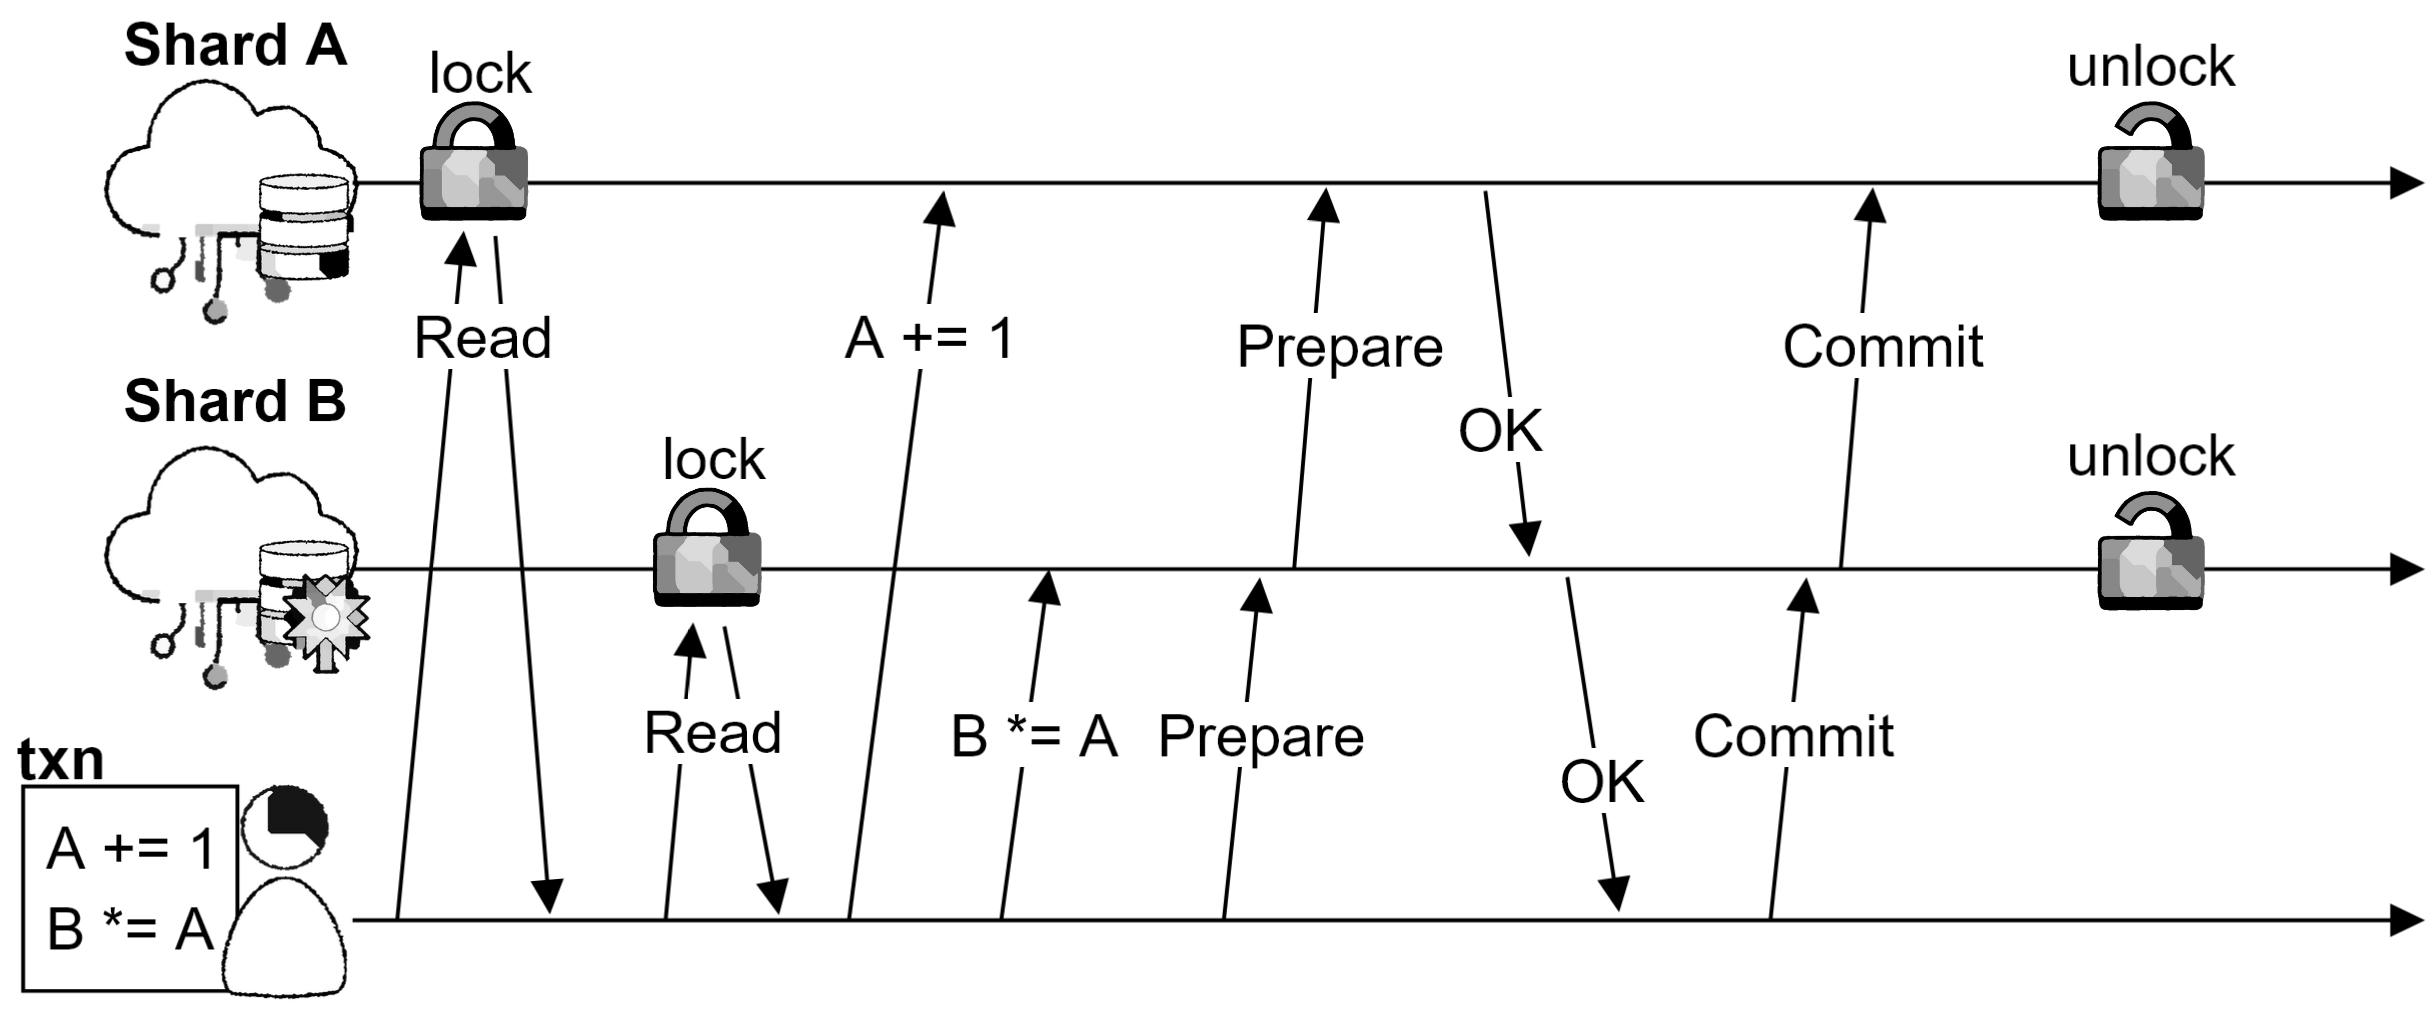
\includegraphics[width=\textwidth]{Sections/span/rw.png}
    \caption{A Read-Write Transaction 2PC Commit in Spanner, where txn is the transaction, $B$'s Paxos leader is the coordinator, and $A$ another participant. First, reads acquire locks, then 2PC begins.
    Commands are sent, and then the \texttt{PREPARE} and \texttt{COMMIT} phases begin, ending with the release of locks.}

\end{figure}

\newpage 


\begin{Example}[MVCC \& TrueTime Evaluation]

    Consider the bellow transactions:
  
 
        \begin{center}
            
           \hspace{-3em} 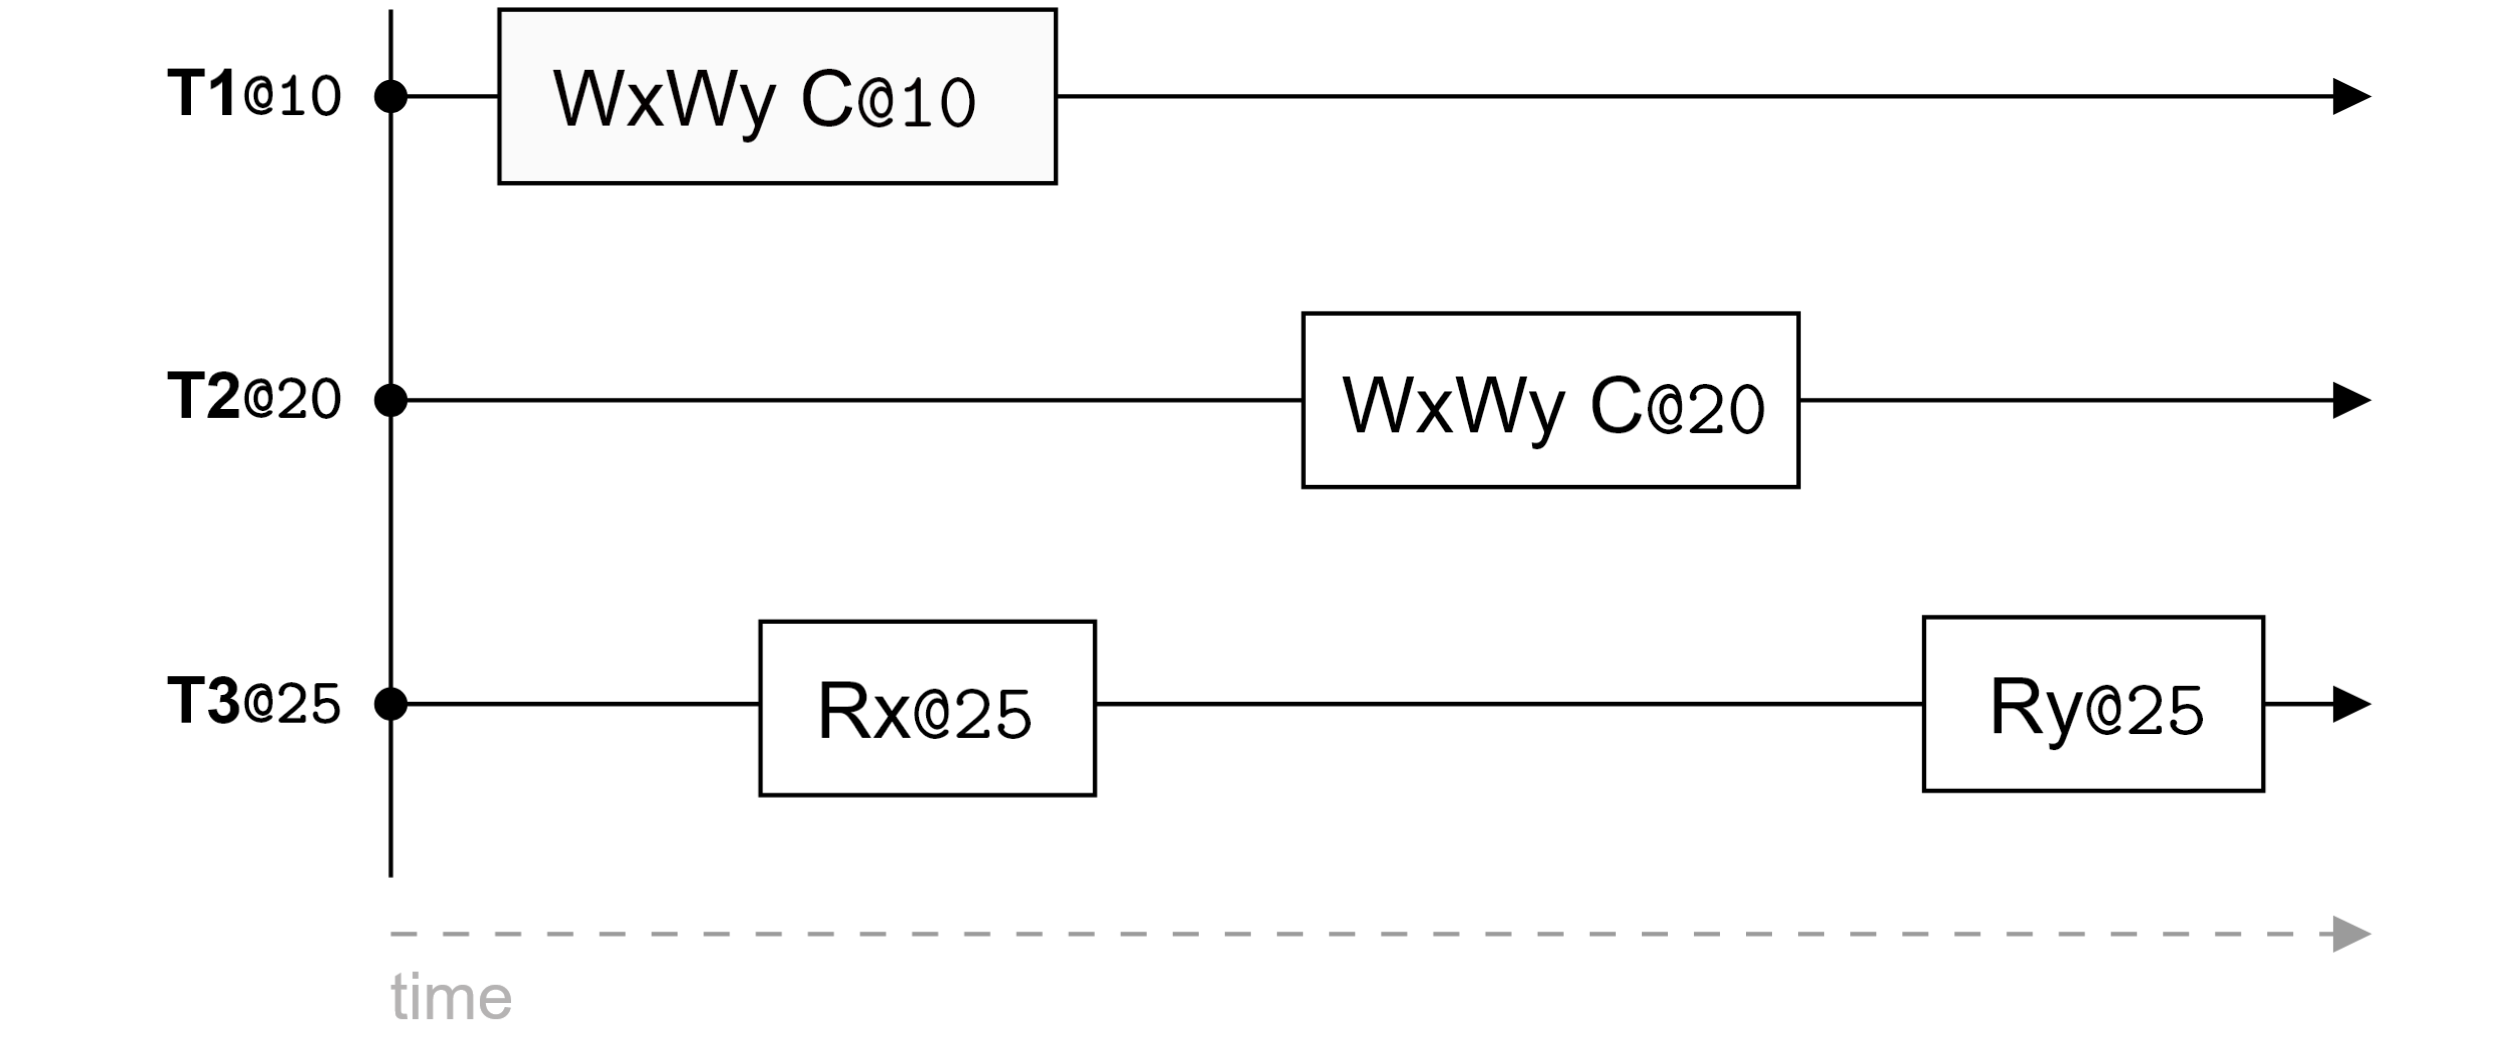
\includegraphics[width=.8\textwidth]{Sections/span/mvcc.png}
        \end{center}
        
    \noindent
    Here we have three transactions, $T_1$, $T_2$, and $T_3$. 
    First we see that $T_1$ make a write request to both keys $x$ and $y$ at timestamp 10.
    Then $T_2$ makes the same request but at timestamp 20. Though it appears $T_3$ is a bit out of sync, reading at 
    time 25. Hence, by the safe time rule, $T_3$ must see a write propagate with a time greater than 25. Now adding TrueTime intervals:
    \begin{center}
            
            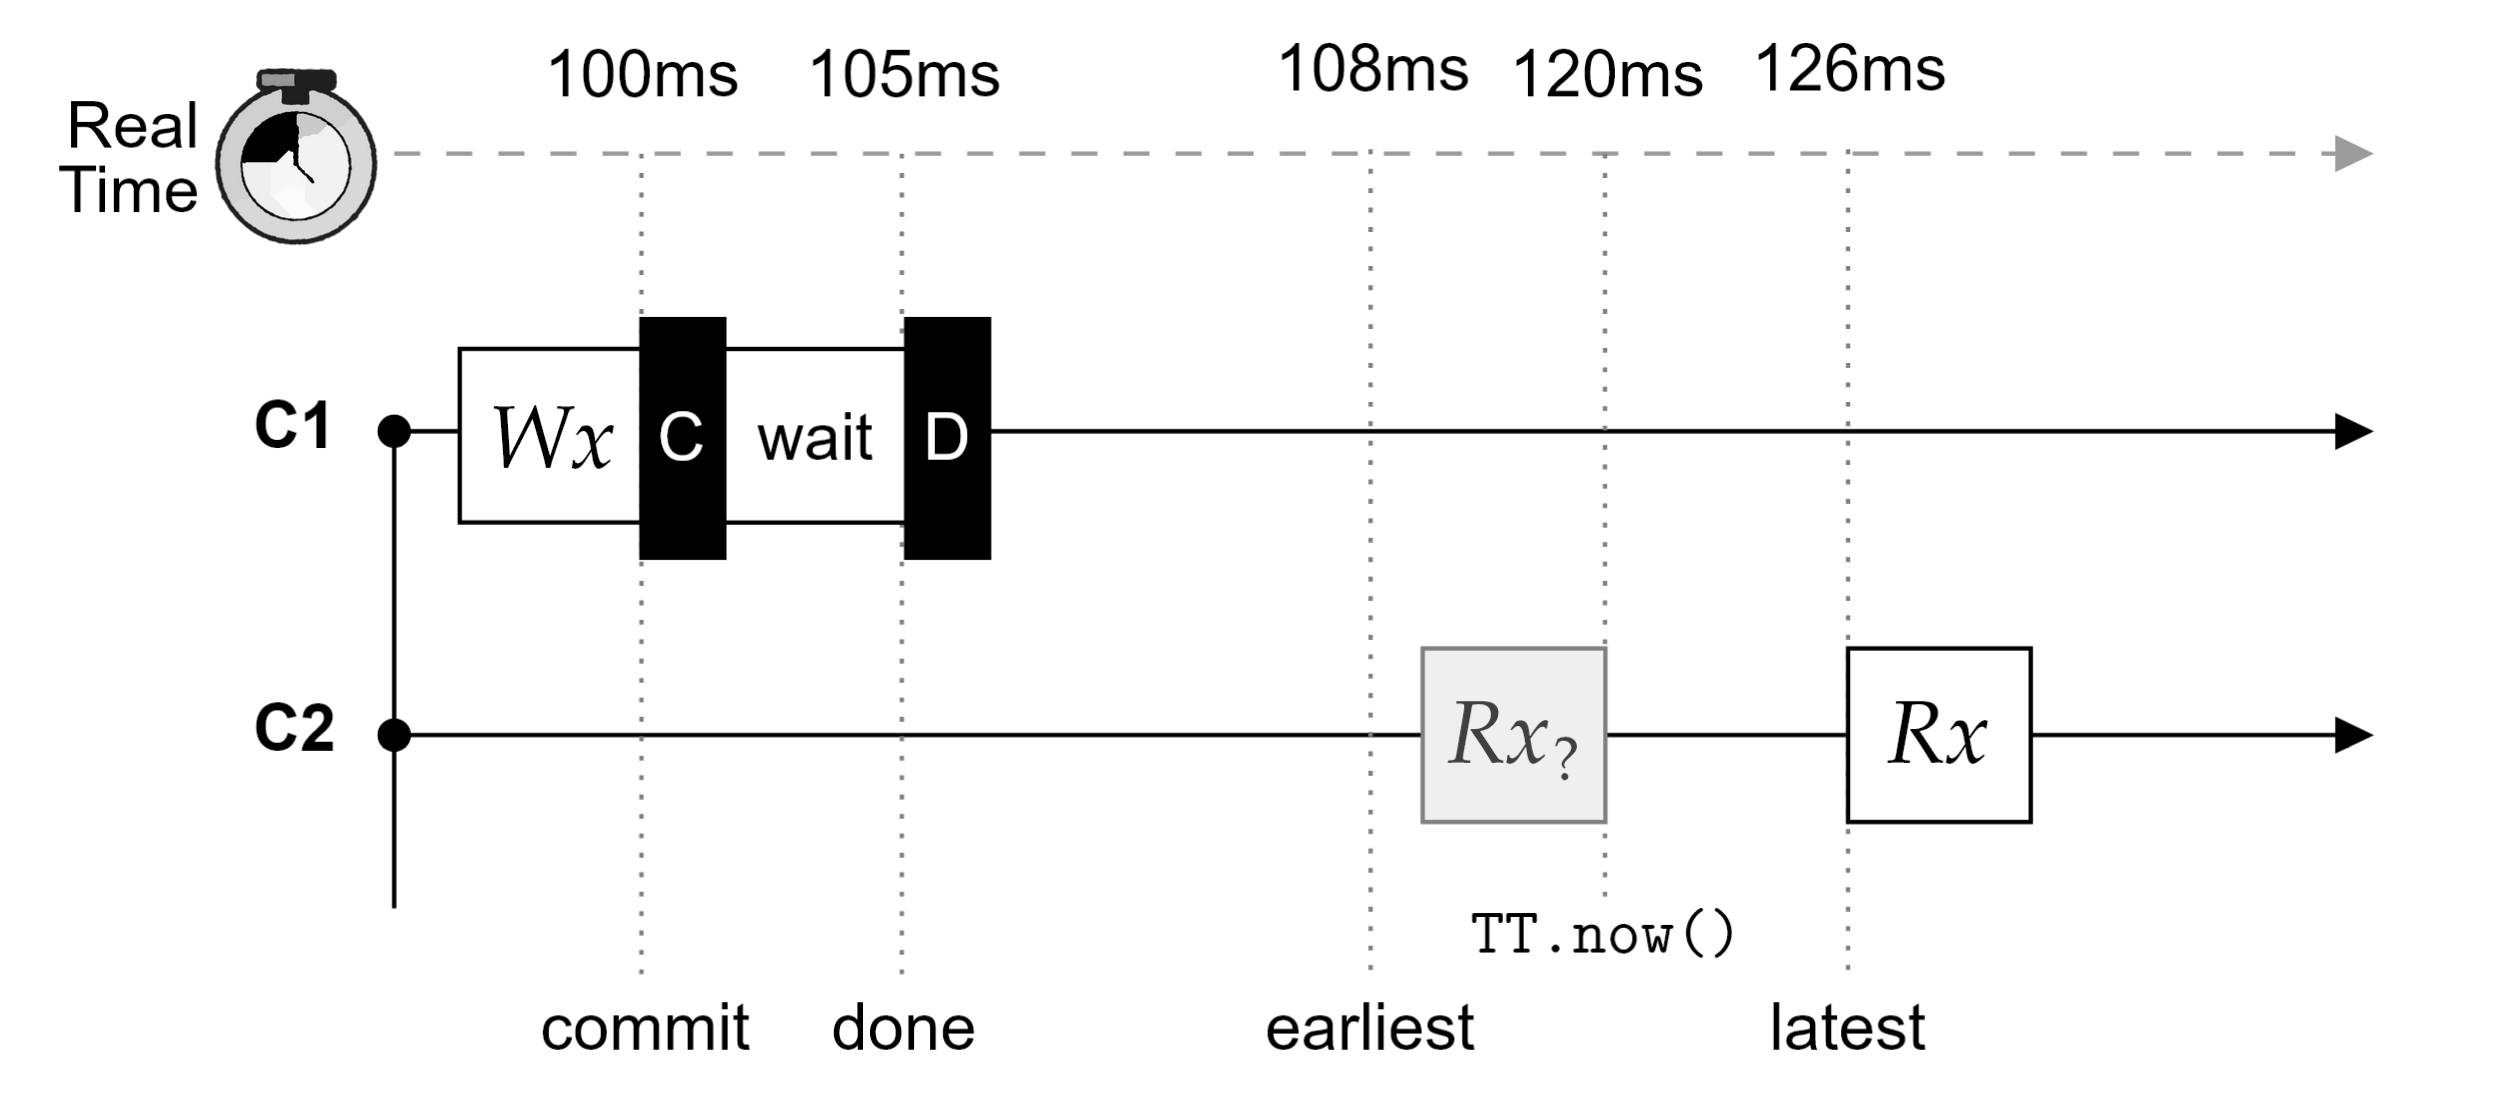
\includegraphics[width=\textwidth]{Sections/span/mvcc_2.png}
        \end{center}
        \noindent
    
    \noindent
    Here client $C_1$ has already prepared the write $Wx$. $C_1$ then sends a commit request at 100 ms, which returns a TrueTime interval of [100ms, 105ms]. The black 
    boxes visualize possible uncertainty intervals. $C_1$ then waits for 5 ms before sending the commit request. On line 2, $C_2$ sends a read request to $x$ at 120 ms.
    They receive a TrueTime interval of [108ms, 126ms]. $C_2$ then waits for 6 ms before sending before attempting to read $x$;
    However, since $C_1$'s commit timestamp is 105ms, $C_2$ must wait for a later commit timestamp, which is typically an insignificant amount of time.
    \end{Example}
            
